\documentclass[10pt,a4paper]{article}

\usepackage[table]{xcolor}
\usepackage{booktabs}
\usepackage{amsmath}
\usepackage{amssymb}
\usepackage{siunitx}
\usepackage[utf8]{inputenc}
\usepackage{pdfpages}
\usepackage[T1]{fontenc}
\usepackage[portuguese]{babel}
\usepackage{graphicx}
\usepackage{eso-pic}
\usepackage{geometry}
\usepackage{setspace}
\usepackage{titlesec}
\usepackage{lmodern}
\usepackage{fancyhdr}
\usepackage{lastpage}
\usepackage{indentfirst}
\usepackage{float}
\usepackage{url}
\usepackage[numbers]{natbib}
\usepackage{subcaption}
% Negrito removido das legendas.
\captionsetup{labelfont=normalfont,textfont=normalfont}
\usepackage{xcolor}
\usepackage{colortbl}
\usepackage{tikz}
\usepackage{comment}
\usepackage{tabularx}
\usepackage[hidelinks]{hyperref}
\usepackage{xurl}
\providecommand{\doi}[1]{\href{https://doi.org/#1}{\nolinkurl{https://doi.org/#1}}}
\providecommand{\preencher}[1]{\textcolor{red}{[#1]}}
\geometry{margin=2.5cm}
\setlength{\headheight}{20pt}
\setstretch{1.25}

\setlength{\parskip}{2pt}
\setlength{\parindent}{20pt}

\fancypagestyle{normal}{
    \fancyhf{}
    \fancyhead[C]{%
        \footnotesize
        \begin{tabular*}{\textwidth}{@{\extracolsep{\fill}} l c r @{}}
             PPFM - Relatório 1 & & 15/10/2026 \\
        \end{tabular*}
    }
    \fancyfoot[R]{Página \thepage}
    \renewcommand{\headrulewidth}{0.4pt}
}
\pagestyle{normal}

\renewenvironment{abstract}{%
  \begin{center}%
    % [negrito removido do título do resumo]
\Large\abstractname\vspace{0.5ex}%
  \end{center}%
}{%
  \par
}

% Coloca cada parte numa página própria e centra o título.
\titleformat{\part}[display]
  {\centering\normalfont}
  {\Large% [negrito removido dos títulos de parte]
\partname\ \thepart}
  {1em}
  {\Huge% [negrito removido dos títulos de parte]
}
% Negrito removido dos títulos de secção.
\titleformat{\section}{\normalfont\Large}{\thesection}{1em}{}
\titleformat{\subsection}{\normalfont\large}{\thesubsection}{1em}{}
\titleformat{\subsubsection}{\normalfont\normalsize}{\thesubsubsection}{1em}{}

\let\originalpart\part
\RenewDocumentCommand{\part}{s o m}{%
  \clearpage
  \thispagestyle{plain}%
  \null\vfill
  \IfBooleanTF{#1}{%
    \originalpart*{#3}%
  }{%
    \IfNoValueTF{#2}{\originalpart{#3}}{\originalpart[#2]{#3}}%
  }%
  \vfill\null
  \clearpage
}

%Começo do documento
\begin{document}

%\nocite{Zhang2025Developing,Bölle2022Modelling,Pishchur2016Recommendations,ppfm-portfolio-2026,astm-d3418-03,protocolo-laboratorial-tp1,madison-group-dsc}

\pagenumbering{Roman}  % Parar contagem de páginas

\begin{titlepage}
    \AddToShipoutPictureBG*{%
        \AtPageLowerLeft{%
            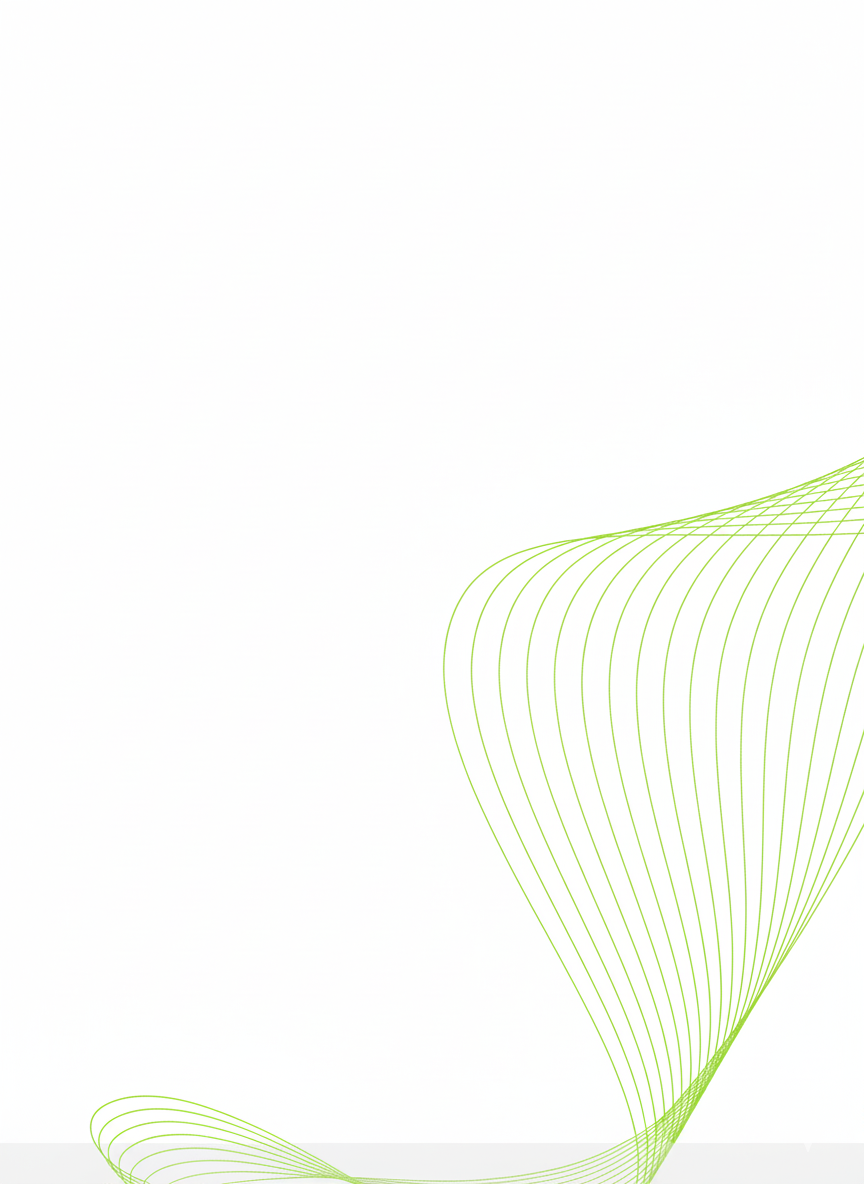
\includegraphics[width=\paperwidth,height=\paperheight,trim=0 41bp 0 0,clip]{Imagens/Capa/Gemini_Generated_Image_mkb5x9mkb5x9mkb5.png}%
        }%
    }

    % Meter logo do DEM
    \begin{figure}[H]
        \centering
\includegraphics[width=0.2\linewidth]{Imagens/Capa/logo_dem.jpg}
    \end{figure}

    \vspace{2\baselineskip}

    % Titulo
    \noindent\huge% [negrito removido: Processamento de Polímeros e Ferramentas Moldantes]
Processamento de Polímeros e Ferramentas Moldantes\\ Relatório 1 - 15/10/2026
    \vspace{\baselineskip}

    % Sub-Título
    \noindent\Large
    \vspace{\baselineskip}

    %Autores
    {\noindent% [negrito removido: Gabriel Ribeiro Nºmec: 113162\\ Leonardo Silva Nºmec: 109040\\ Flávio Terrível Nºmec: 113156\\ Pedro Pinto Nºmec: 120169\\ Rafael Rodrigues Nºmec: 111621\\ Bruno...Nºmec:]
    Grupo 3:
    \begin{itemize}
        \item Gabriel Ribeiro Nºmec: 113162
        \item Leonardo Silva Nºmec: 109040
        \item Flávio Terrível Nºmec: 113156
        \item Pedro Pinto Nºmec: 120169
        \item Rafael Rodrigues Nºmec: 111621
        \item Bruno Loureiro Nºmec: 108350
    \end{itemize}}


    \vspace{3\baselineskip}

    %\begin{abstract}
    %\small

    %\large
    %\vspace{5pt}
    %\small
    %\noindent



    % [negrito removido: comando vazio]

    %\end{abstract}

    \large

    \vspace{35pt}

    \clearpage
\end{titlepage}

\newpage



\begingroup
\small
\tableofcontents
\endgroup

\newpage
\phantomsection
\addcontentsline{toc}{section}{Lista de Figuras}
\listoffigures
\phantomsection
\addcontentsline{toc}{section}{Lista de Tabelas}
\listoftables





\newpage



\pagenumbering{arabic} % Começar contagem de páginas


%%%%%%%%%%%%%%%%%%%%%%%%%%%%%%%%%%%%%%%%%%%%%%%%%%%

\section{Artigo e Previsões}


\subsection{Leitura crítica}
O artigo de Zhang et al. (2026) investiga o inchamento anisotrópico do extrudido durante a extrusão de polímeros através de uma fieira de fenda de geometria retangular. O problema abordado deve-se ao facto de os modelos existentes, embora expliquem o inchamento do extrudido com base na recuperação elástica do material, não descreverem completamente as diferenças de expansão observadas nas várias direções deste tipo de fieiras. Neste contexto, os autores propõem desenvolver um modelo matemático que relaciona a distribuição local da velocidade do escoamento com a distribuição do inchamento do extrudido. A consistência do modelo é posteriormente avaliada através da comparação das suas previsões com resultados de simulações CFD realizadas no ANSYS Polyflow, recorrendo ao modelo constitutivo da Lei da Potência. Na formulação do modelo matemático, os autores assumem um fluido incompressível, um escoamento laminar completamente desenvolvido, condições isotérmicas e uma fieira idealmente infinita em largura.

O domínio computacional utilizado nas simulações CFD encontra-se dividido em duas regiões. A primeira corresponde à zona confinada da matriz, onde o polímero escoa no interior do canal da fieira. Esta região permite estabelecer a distribuição de velocidades à saída da matriz, sendo aplicada uma condição de não deslizamento nas paredes, que impõe velocidade nula do fluido junto às mesmas. A segunda região corresponde à zona de escoamento em superfície livre, situada imediatamente após a saída da fieira. Nesta região, o polímero deixa de estar confinado pelas paredes da matriz, ficando livre para se deformar e expandir. É, portanto, nesta zona que se simula e avalia o fenómeno de inchamento do extrudido.

Importa, contudo, salientar que os resultados obtidos não constituem uma validação física do inchamento viscoelástico de polímeros reais. Nas simulações CFD, os autores recorrem ao modelo da Lei da Potência, que permite representar o comportamento não newtoniano e pseudoplástico do fluido, mas não tem em conta a sua natureza viscoelástica, nomeadamente a acumulação e posterior recuperação das tensões elásticas durante o escoamento na fieira. Assim, a comparação entre o modelo matemático e os resultados numéricos permite avaliar essencialmente a consistência geométrica e cinemática da abordagem proposta, não reproduzindo integralmente o inchamento real dos polímeros fundidos. Adicionalmente, as simulações são realizadas em condições isotérmicas, não sendo considerados os efeitos dos gradientes de temperatura sobre o escoamento e a viscosidade.

Outra limitação importante vem da aproximação de largura infinita adotada no modelo matemático, que pressupõe uma distribuição de velocidades uniforme na direção da largura da fieira, desprezando os efeitos das paredes laterais. Contudo, nas simulações CFD tridimensionais, que consideram uma condição de não deslizamento nas paredes, verifica-se uma diminuição local da velocidade nas regiões próximas das mesmas. Esta diferença provoca um afastamento entre as previsões teóricas e os resultados numéricos, particularmente na zona periférica da fieira. Os autores identificam que, nas regiões próximas das extremidades, os erros podem ultrapassar 30\%, sobretudo na componente do deslocamento segundo a direção da espessura. 



\subsection{Previsões fundamentadas}

\textbf{P1. Onde se esperam as maiores taxas de deformação e porquê?} 

As maiores taxas de deformação vão surgir nas paredes da zona confinada da matriz, com o pico máximo a acontecer nas arestas de saída. Dentro da fieira, o polímero adere à parede devido à condição de não escorregamento, o que leva a velocidade local a zero e empurra o gradiente transversal para o limite máximo. Exatamente na aresta de saída, o fluido passa de repente desse bloqueio físico para a zona de superfície livre. Este salto cria um ponto crítico onde o polímero sofre a variação de velocidade mais brusca de toda a simulação para se conseguir reorganizar. \\


\textbf{P2. O Caso M deverá exigir uma queda de pressão superior ou inferior à obtida no Caso R? Justifique. }

O Caso M vai precisar de uma queda de pressão maior do que a do Caso R. Embora o polipropileno Moplen HP648T tenha um índice de consistência mais baixo ($K=$900 Pa$\cdot$s face aos 1000 Pa$\cdot$s do Caso R), o seu índice de comportamento ($n=$0,64 contra $n=$0,60) mostra que é um material com menor reofluidificação. Isto significa que, nas taxas de corte reais que vão acontecer na extrusão, este polímero perde menos viscosidade do que o fluido de referência. Como mantém uma viscosidade aparente mais alta, o escoamento tem mais resistência e exige uma maior pressão para conseguir manter o caudal de 200 mm$^3$/s. \\


\textbf{P3. A alteração da reologia deverá modificar a deformação geométrica calculada do extrudido? Em que sentido? }

A mudança na reologia aumentará o inchamento do extrudido no Caso M. Uma vez que o modelo não considera a elasticidade do polímero, a expansão simulada não é o relaxamento viscoelástico, mas sim o resultado de um reajuste cinemático. Por ter menor reofluidificação, este material desenvolve um perfil de velocidades mais parabólico dentro da matriz. À saída, a necessidade de conservar o caudal obriga esse perfil a uniformizar-se na superfície livre. Sendo o perfil inicial do Caso M mais acentuado, a sua uniformização exige deslocar mais massa do centro para as laterais, resultando numa expansão geométrica superior.


% =====================================================================
% 2 - Modelo Numérico
% Rascunho de apoio (IA) - o grupo deve rever e reescrever antes de incluir.
% Valores retirados do enunciado, da ficha reológica (Grupo 3) e dos
% ficheiros polyflow.lst dos Casos R (PFL) e M (PFL-1).
% Campos a vermelho (\preencher) = confirmar no setup do Polyflow.
% =====================================================================

\section{Modelo Numérico}
\label{sec:modelo}

\subsection{Domínio, Geometria e Malha}
\label{subsec:dominio}

A geometria reproduz o caso de Zhang et al.~\cite{Zhang2026Anisotropic}: fieira de fenda retangular com largura $W = 20$~mm, espessura $2H = 2$~mm, troço confinado $L = 20$~mm e região de jato livre $L_F = 40$~mm. Explorando as duas simetrias da secção, simula-se apenas um quarto do domínio ($10 \times 1 \times 60$~mm), composto por dois corpos: o troço confinado da matriz ($z \in [0,20]$~mm) e o jato livre ($z \in [20,60]$~mm). Os dois corpos formam um único componente com \textit{Share Topology}, pelo que a interface em $z = 20$~mm é interna e a malha é conforme.

Foi utilizada a malha hexaédrica fornecida pela equipa docente (\textit{MultiZone}, dimensão de elemento de 0,3~mm), com 27\,336 elementos e 35\,350 nós. Não foram introduzidas alterações à geometria, à malha nem às \textit{Named Selections}; os Casos R e M partilham exatamente a mesma discretização. A malha do artigo é graduada (10 elementos na altura, 40 na largura, 30 no troço confinado e 35 no jato livre, com refinamento junto à saída), ao passo que a malha fornecida é uniforme, pelo que os resultados não são comparáveis em detalhe com os do artigo, sobretudo junto à aresta de saída.

\subsection{Hipóteses do Regime}
\label{subsec:hipoteses}

Em ambos os casos resolve-se o problema de Navier--Stokes 3D com as seguintes hipóteses, coerentes com o caso de referência:
\begin{itemize}
    \item escoamento estacionário e isotérmico (não se resolve a equação da energia);
    \item fluido incompressível e newtoniano generalizado, isto é, puramente viscoso, sem memória elástica (o Polyflow usa um fator de compressibilidade relativa de $10^{-2}$ apenas para estabilizar o cálculo da pressão, sem alterar a hipótese física);
    \item forças de inércia e gravidade desligadas na configuração do Polyflow (a massa volúmica no \textit{setup} é 1~kg/m$^3$, valor sem efeito com a inércia desligada). A hipótese é adequada ao escoamento lento de um fundido: com $\rho \approx 760$~kg/m$^3$ (ficha), velocidade média $\dot{V}/(W\,2H) \approx 0{,}02$~m/s, diâmetro hidráulico $\approx 4$~mm e $\eta \approx 200$~Pa$\cdot$s, obtém-se $Re \approx 3 \times 10^{-4}$;
    \item aderência total à parede da matriz e superfície livre sem tensão superficial.
\end{itemize}
A hipótese de fluido puramente viscoso é a mais relevante para a interpretação dos resultados: a deformação do extrudido calculada resulta apenas do rearranjo cinemático do perfil de velocidades à saída da matriz, e não da recuperação elástica do polímero.

\subsection{Modelo Reológico (Casos R e M)}
\label{subsec:reologia}

A viscosidade é descrita pela lei de potência, que no Polyflow tem a forma
\begin{equation}
    \eta(\dot{\gamma}) = \mathit{fac}\,(t_{\mathrm{nat}}\,\dot{\gamma})^{\mathit{expo}-1} = K\,\dot{\gamma}^{\,n-1},
    \label{eq:leipotencia}
\end{equation}
com $\mathit{fac} = K$, $\mathit{expo} = n$ e tempo de referência $t_{\mathrm{nat}} = 1$~s, de modo que $\mathit{fac}$ tem o valor numérico de $K$ em Pa$\cdot$s$^n$. O Caso M foi criado a partir de uma cópia do Caso R, alterando apenas $\mathit{fac}$ e $\mathit{expo}$ (Tabela~\ref{tab:reologia}).

\begin{table}[H]
    \centering
    \caption{Parâmetros reológicos dos Casos R e M (lei de potência).}
    \label{tab:reologia}
    \begin{tabular}{lcc}
        \toprule
        & Caso R (referência) & Caso M (Moplen HP648T) \\
        \midrule
        Material & Fluido de referência~\cite{Zhang2026Anisotropic} & PP homopolímero nucleado \\
        Temperatura associada & -- & 220~°C \\
        $K$ ($\mathit{fac}$) [Pa$\cdot$s$^n$] & 1000 & 900 \\
        $n$ ($\mathit{expo}$) [--] & 0,60 & 0,64 \\
        $t_{\mathrm{nat}}$ [s] & 1 & 1 \\
        Intervalo de validade de $\dot{\gamma}$ [s$^{-1}$] & -- & 60 -- 500 \\
        \bottomrule
    \end{tabular}
\end{table}

Os parâmetros do Caso M foram confirmados contra os valores de controlo da ficha~\cite{FichaMoplen}: pela Eq.~\ref{eq:leipotencia} obtém-se $\eta = 206$~Pa$\cdot$s a 60~s$^{-1}$ e $\eta = 96$~Pa$\cdot$s a 500~s$^{-1}$, iguais aos tabelados. Fora do intervalo de 60 a 500~s$^{-1}$, a utilização da lei corresponde a extrapolação, o que será avaliado na Secção~\ref{sec:casos}. O artigo usa $K = 1000$~Pa$\cdot$s$^n$ e $n = 0{,}5$~\cite{Zhang2026Anisotropic}; o Caso R usa o mesmo $K$ mas $n = 0{,}6$, valor fixado no enunciado, pelo que a reprodução do caso de Zhang é válida para a geometria e para $K$, não para $n$. Como $n < 0{,}75$ nos dois casos, o guia do enunciado indica que o Polydata emite um aviso ao introduzir $\mathit{expo}$, o que motiva a estratégia de convergência descrita na Secção~\ref{subsec:numerica}.

\subsection{Condições de Fronteira}
\label{subsec:fronteiras}

As condições de fronteira foram atribuídas às \textit{Named Selections} fornecidas, iguais nos dois casos (Tabela~\ref{tab:fronteiras}).

\begin{table}[H]
    \centering
    \caption{Condições de fronteira aplicadas nos Casos R e M.}
    \label{tab:fronteiras}
    \begin{tabularx}{\textwidth}{>{\raggedright\arraybackslash}p{2.5cm} >{\raggedright\arraybackslash}p{4cm} X}
        \toprule
        \textit{Named Selection} & Condição & Significado físico \\
        \midrule
        INLET ($z = 0$) & Escoamento completamente desenvolvido & Caudal imposto $Q = 2 \times 10^{-7}$~m$^3$/s (200~mm$^3$/s no quarto do domínio); o perfil de entrada é calculado pelo Polyflow como escoamento de canal 2D na secção de entrada. \\
        \midrule
        DIEWALL & Parede, $\mathbf{v} = \mathbf{0}$ & Aderência total do fundido à parede do troço confinado. \\
        \midrule
        FREESURFACE & Superfície livre & Tensões nulas e condição cinemática $\mathbf{v}\cdot\mathbf{n} = 0$; a posição da superfície é incógnita, ficando imposta apenas na aresta comum com DIEWALL (saída da matriz). \\
        \midrule
        OUTLET ($z = 60$~mm) & Fronteira livre de tensões ($\boldsymbol{\sigma}\cdot\mathbf{n} = \mathbf{0}$), como no artigo~\cite{Zhang2026Anisotropic} \preencher{confirmar no setup} & Secção final do extrudido, onde se medem $B_W$ e $B_H$. \\
        \midrule
        SYMETRYX, SYMETRYY & Plano de simetria & $v_n = 0$ e tensão tangencial nula; permitem simular apenas 1/4 do domínio. \\
        \bottomrule
    \end{tabularx}
\end{table}

\subsection{Configuração Numérica}
\label{subsec:numerica}

Seguiu-se a configuração trabalhada nas aulas, sem alterações adicionais. Para garantir a convergência com $n < 0{,}75$, ativou-se a opção \textit{Enable evolution on moving boundaries}, que introduz progressivamente a superfície livre fazendo variar o parâmetro de evolução $S$ de 0 a 1 (passo inicial $\Delta S = 0{,}01$, mínimo $10^{-4}$, máximo $0{,}25$). A lei de viscosidade é resolvida pelo método de Newton e a deformação da malha do jato livre é acompanhada pelo algoritmo de remalhagem Optimesh~3D. Em cada passo considera-se a convergência atingida quando a variação relativa da solução é inferior a $10^{-3}$, critério definido pela equipa docente.

Nos dois casos a evolução chegou a $S = 1$ em 10 passos, sem nenhum passo falhado, pelo que não foi necessário ativar as iterações de Picard. Os tempos de cálculo foram de 409~s (Caso R) e 336~s (Caso M). Estas opções afetam apenas a estabilidade do processo numérico e não alteram o modelo reológico, o caudal imposto nem as condições físicas.



\section{Caso R e Caso M}
\label{sec:casos}

A extração de resultados seguiu a mesma metodologia nos dois casos: a queda de pressão foi calculada por $\Delta p = \bar{p}_{\mathrm{ent}} - \bar{p}_{\text{saída}}$, com médias de área em $z = 0$~mm e $z = 20$~mm, e os rácios de inchamento na secção final ($z = 60$~mm) por $B_W = x_{\max}/(W/2)$ e $B_H = y_{\max}/H$, com $W/2 = 10$~mm e $H = 1$~mm.

\subsection{Verificação Numérica e Controlo de Coerência Física}
\label{subsec:verificacao}

A estratégia de evolução convergiu com sucesso em ambos os casos ($S = 1$ em 10 passos, sem falhas e com resíduo relativo inferior a $10^{-3}$). A conservação de caudal foi verificada pelo erro $\varepsilon_Q = 0{,}009\,\%$ (Tabela~\ref{tab:verificacao}), correspondente a um fluxo residual numérico de $1{,}8 \times 10^{-11}$~m$^3$/s na superfície livre.

\begin{table}[H]
    \centering
    \small
    \caption{Verificação numérica dos Casos R e M.}
    \label{tab:verificacao}
    \begin{tabular}{lccccc}
        \toprule
        Caso & $|Q_{\mathrm{in}}|$ [m$^3$/s] & $|Q_{\mathrm{out}}|$ [m$^3$/s] & $\varepsilon_Q$ [\%] & Passos (falhados) & Tempo [s] \\
        \midrule
        R & $2{,}000 \times 10^{-7}$ & $1{,}999 \times 10^{-7}$ & 0,009 & 10 (0) & 409 \\
        M & $2{,}000 \times 10^{-7}$ & $1{,}999 \times 10^{-7}$ & 0,009 & 10 (0) & 336 \\
        \bottomrule
    \end{tabular}
\end{table}

A coerência física foi verificada confrontando $\Delta p$ com a solução analítica unidimensional para escoamento desenvolvido de um fluido da lei de potência entre placas paralelas infinitas:
\begin{equation}
    \Delta p_{\mathrm{1D}} = \frac{2L}{h}K\dot{\gamma}_w^n, \quad \text{com} \quad \dot{\gamma}_w = \left(\frac{2n+1}{3n}\right)\frac{6Q_{\mathrm{total}}}{W h^2}.
\end{equation}
Nesta expressão, $h = 2$~mm, $W = 20$~mm, $L = 20$~mm e $Q_{\mathrm{total}} = 4Q = 8 \times 10^{-7}$~m$^3$/s. A formulação analítica fornece $263{,}0$~kPa (R) e $276{,}2$~kPa (M). Os valores do Polyflow ($287{,}4$~kPa e $301{,}5$~kPa) são cerca de 9\,\% superiores devido ao atrito tridimensional introduzido pelas paredes laterais finitas ($W/(2H) = 10$) e ao rearranjo cinemático à saída ($z = 20$~mm). A razão entre casos ($\Delta p_M/\Delta p_R$) é semelhante nos dois métodos: 1,049 no Polyflow e 1,050 na solução analítica, validando a coerência física do modelo.

\subsection{Campos de Escoamento e Deformação do Extrudido}
\label{subsec:resultados}

\paragraph{Queda de pressão na matriz.} A perda de carga calculada no troço confinado ($z \in [0,20]$~mm) foi de $\Delta p_R = 287{,}4$~kPa no Caso R e de $\Delta p_M = 301{,}5$~kPa no Caso M. Para o mesmo caudal imposto de 200~mm$^3$/s no quarto do domínio, o polipropileno (Caso M) exige um acréscimo de pressão de 4,9\,\% face ao fluido de referência.

\paragraph{Distribuição de velocidades.} A Figura~\ref{fig:velocidades} apresenta os mapas de contorno da velocidade no plano médio de simetria ($Y = 0$), com uma escala comum de 0 a 0,035~m/s. Dentro da matriz ($z \in [0,20]$~mm), observa-se um perfil desenvolvido, com velocidade máxima no núcleo central ($X = 0$), atingindo $v_{\max} \approx 0,034$~m/s em ambos os casos e decaindo até zero na parede lateral ($X = 10$~mm). A jusante da aresta de saída ($z > 20$~mm), o núcleo central desacelera e a camada periférica acelera, estabelecendo um escoamento em bloco (\textit{plug flow}) com velocidade aproximadamente uniforme de 0,020~m/s ao longo do jato livre, coerente com o caudal volumétrico e a secção do extrudido.

\begin{figure}[htbp]
    \centering
    \begin{subfigure}[b]{0.48\textwidth}
        \centering
        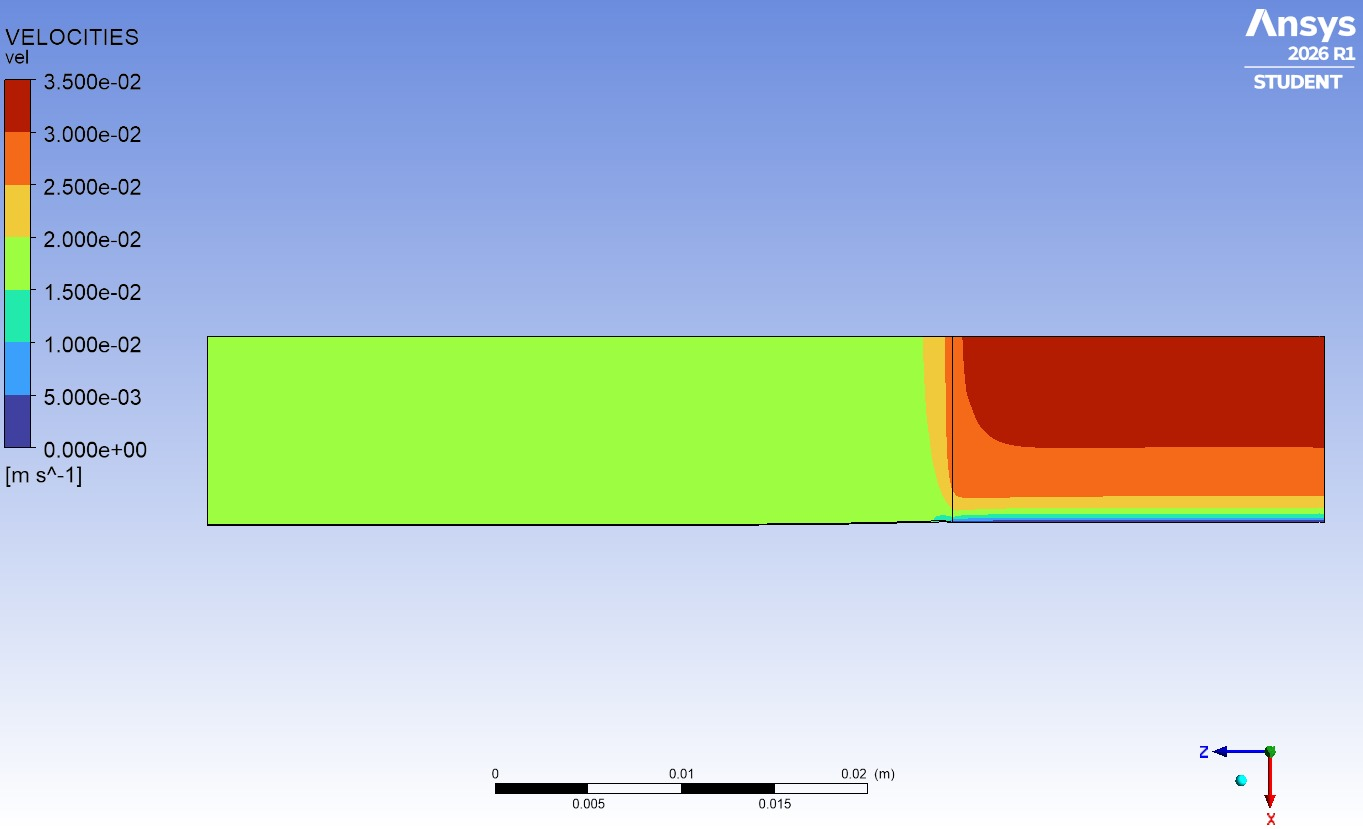
\includegraphics[width=\textwidth]{Imagens/vel_R.jpeg}
        \caption{Caso R (referência)}
        \label{fig:vel_R}
    \end{subfigure}
    \hfill
    \begin{subfigure}[b]{0.48\textwidth}
        \centering
        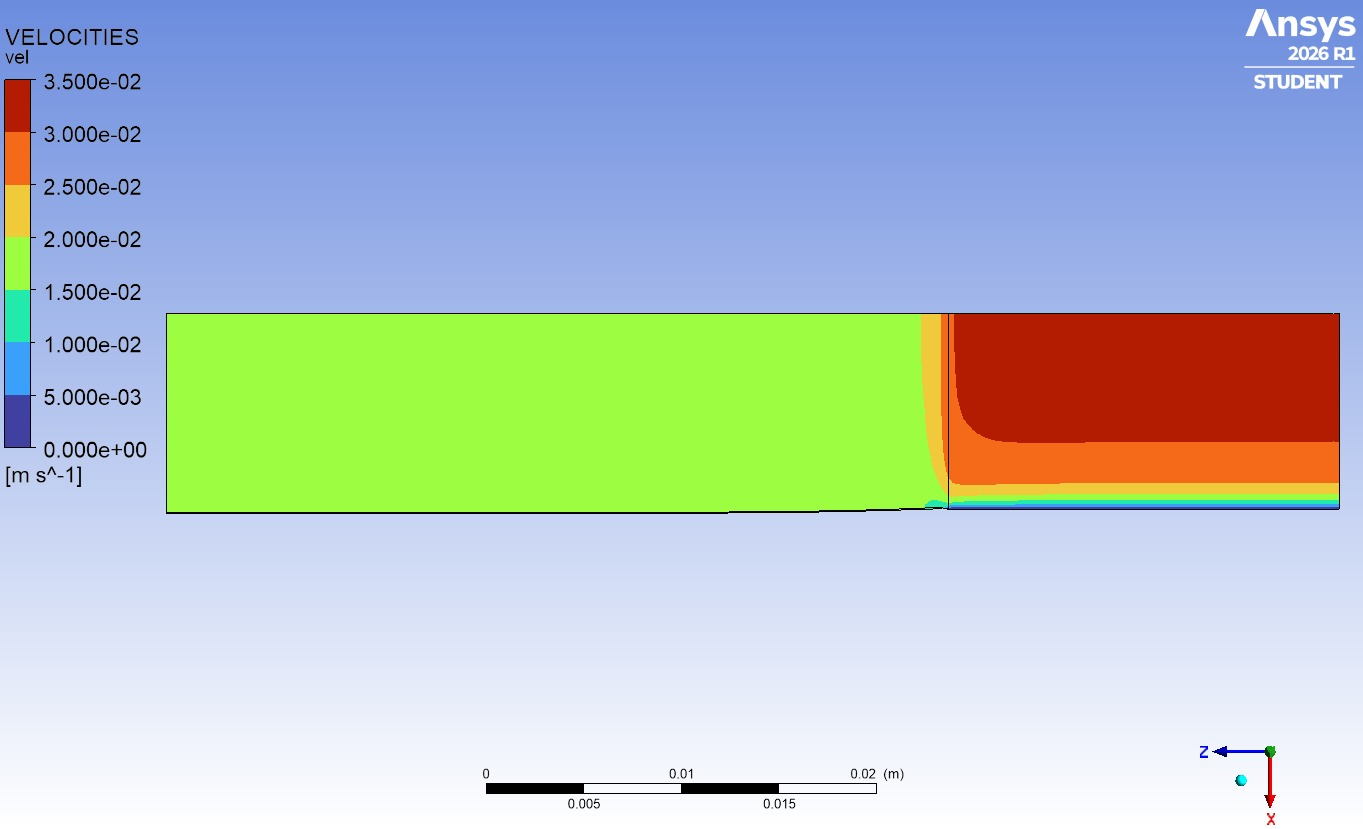
\includegraphics[width=\textwidth]{Imagens/vel_M.jpeg}
        \caption{Caso M (Moplen HP648T)}
        \label{fig:vel_M}
    \end{subfigure}
    \caption{Distribuição de velocidades no plano de simetria $Y = 0$: (a) Caso R e (b) Caso M (escala comum de 0 a 0,035~m/s).}
    \label{fig:velocidades}
\end{figure}

\paragraph{Taxa de deformação.} A Figura~\ref{fig:deformacao} ilustra a distribuição da taxa de corte local ($\dot{\gamma}$) à superfície do domínio, com escala comum de 0 a 90~s$^{-1}$. Na parede da matriz (DIEWALL), a taxa de deformação varia entre 5,5 e 81,5~s$^{-1}$ no Caso R e entre 5,7 e 80,3~s$^{-1}$ no Caso M. O valor médio na secção anterior à saída ($z = 19$~mm) é, respetivamente, 29,1~s$^{-1}$ e 29,3~s$^{-1}$. A aresta de saída da fieira ($z = 20$~mm) constitui a região crítica do domínio, registando-se aí uma descontinuidade abrupta decorrente da transição da condição de não escorregamento para a superfície livre sem tensões. No jato livre, a uniformização do perfil anula os gradientes espaciais de velocidade, fazendo a taxa de deformação decair rapidamente para zero ($\dot{\gamma} \approx 0$~s$^{-1}$).

\begin{figure}[htbp]
    \centering
    \begin{subfigure}[b]{0.48\textwidth}
        \centering
        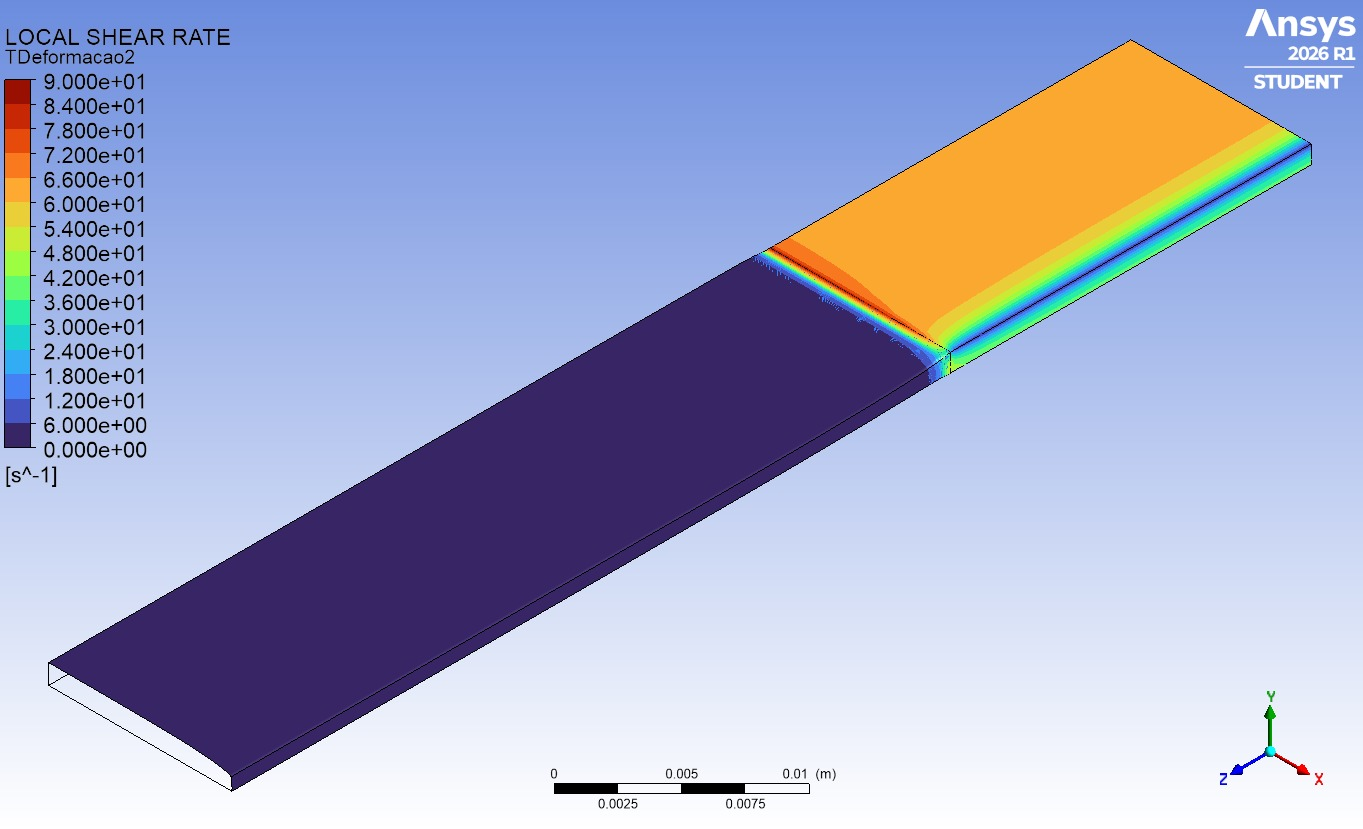
\includegraphics[width=\textwidth]{Imagens/shear_R.jpeg}
        \caption{Caso R (referência)}
        \label{fig:shear_R}
    \end{subfigure}
    \hfill
    \begin{subfigure}[b]{0.48\textwidth}
        \centering
        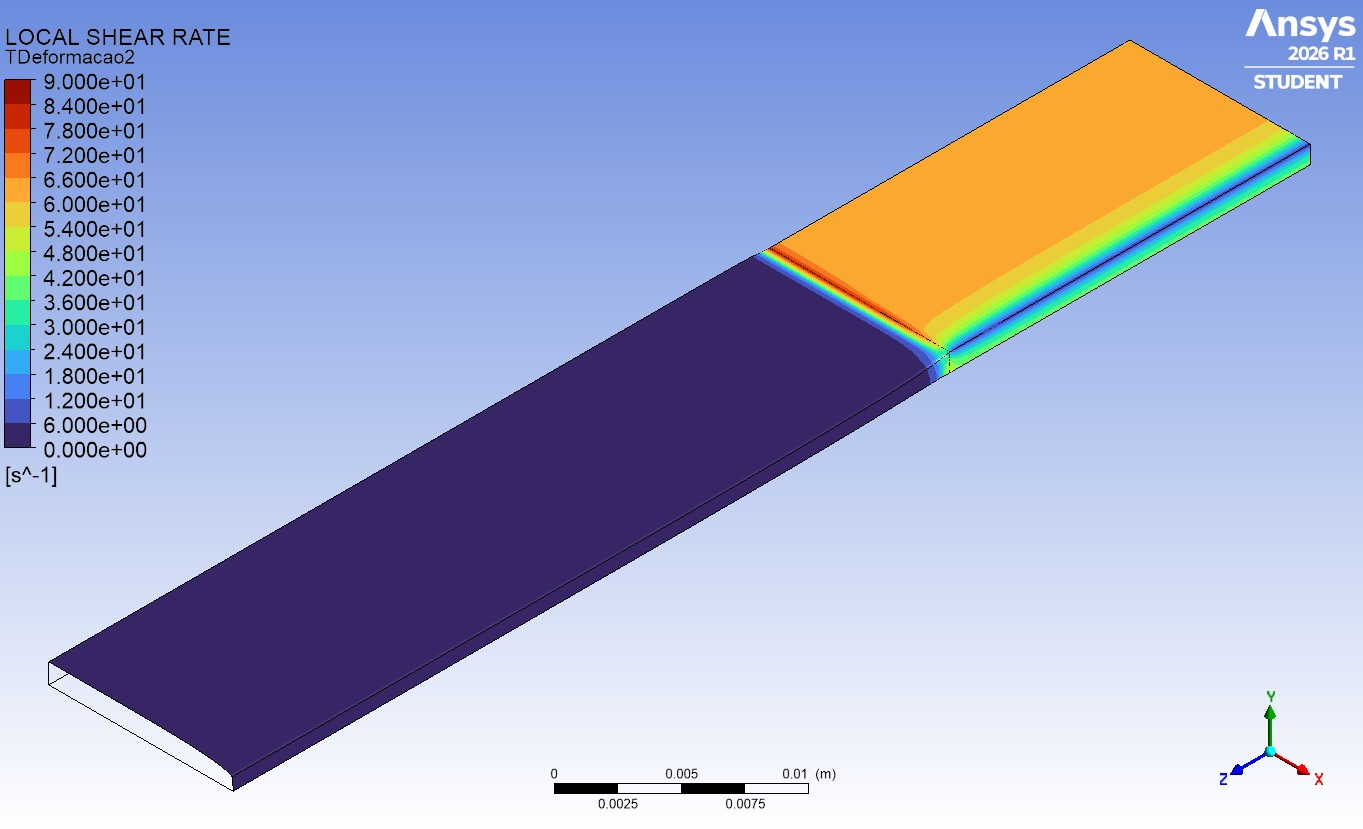
\includegraphics[width=\textwidth]{Imagens/shear_M.jpeg}
        \caption{Caso M (Moplen HP648T)}
        \label{fig:shear_M}
    \end{subfigure}
    \caption{Distribuição da taxa de deformação local ($\dot{\gamma}$): (a) Caso R e (b) Caso M (escala comum de 0 a 90~s$^{-1}$).}
    \label{fig:deformacao}
\end{figure}

\paragraph{Deformação geométrica do extrudido.} A Figura~\ref{fig:inchamento} compara a geometria da secção transversal na saída livre ($z = 60$~mm) com a secção nominal da fieira ($10$~mm $\times 1$~mm). Na secção final, mediram-se os rácios de inchamento $B_W = 1{,}017$ e $B_H = 1{,}096$ para o Caso R, e $B_W = 1{,}023$ e $B_H = 1{,}110$ para o Caso M. Em ambos os fluidos constata-se um inchamento viscoso fortemente anisotrópico: a expansão na espessura ($B_H - 1$, cerca de 9,6\,\% em R e 11,0\,\% em M) é cerca de cinco a seis vezes superior à expansão na largura ($B_W - 1$, cerca de 1,7\,\% em R e 2,3\,\% em M). O bordo superior apresenta uma curvatura acentuada nos cantos exteriores, associada ao efeito tridimensional das paredes laterais da fieira.

\begin{figure}[htbp]
    \centering
    \begin{subfigure}[b]{0.48\textwidth}
        \centering
        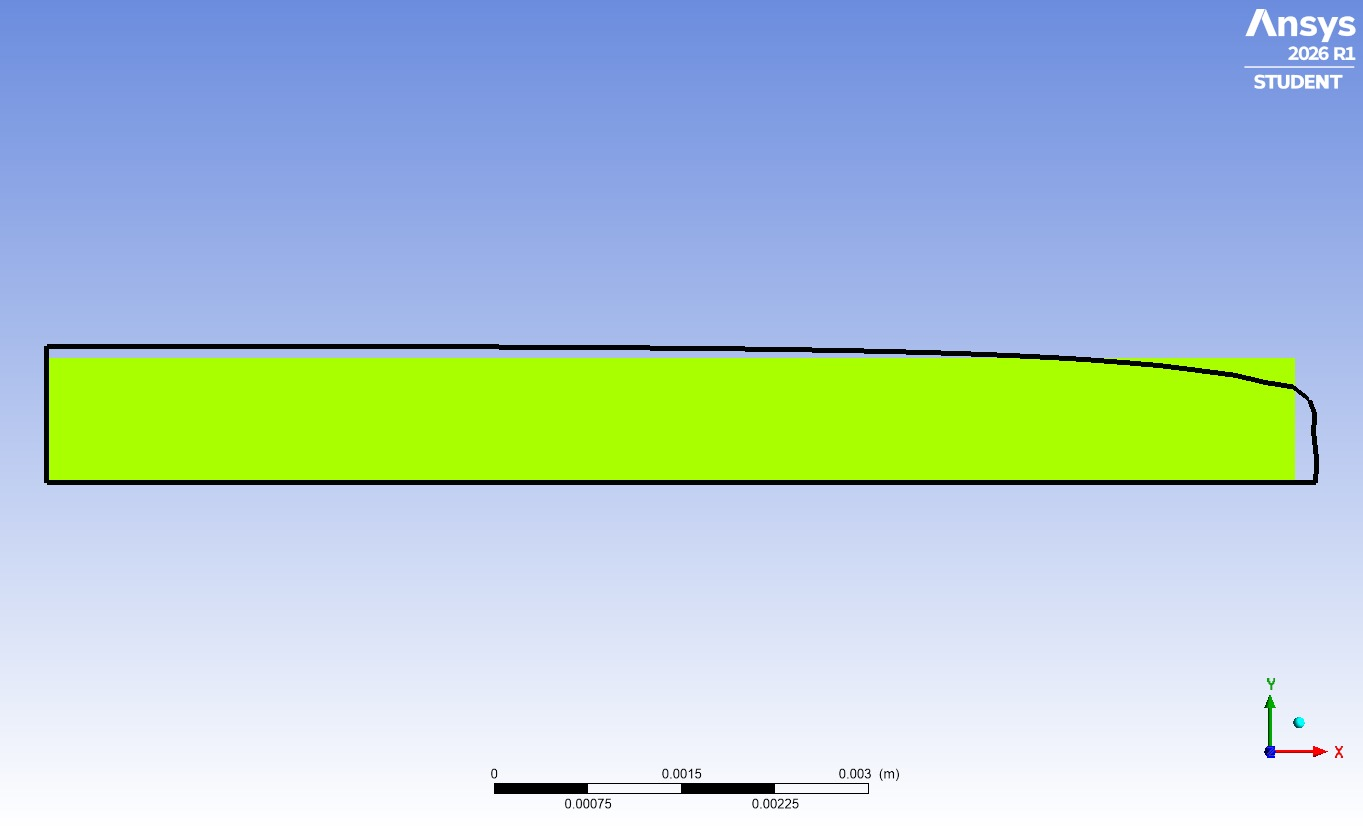
\includegraphics[width=\textwidth]{Imagens/perfil_R.jpeg}
        \caption{Caso R ($B_W = 1,017$; $B_H = 1,096$)}
        \label{fig:perfil_R}
    \end{subfigure}
    \hfill
    \begin{subfigure}[b]{0.48\textwidth}
        \centering
        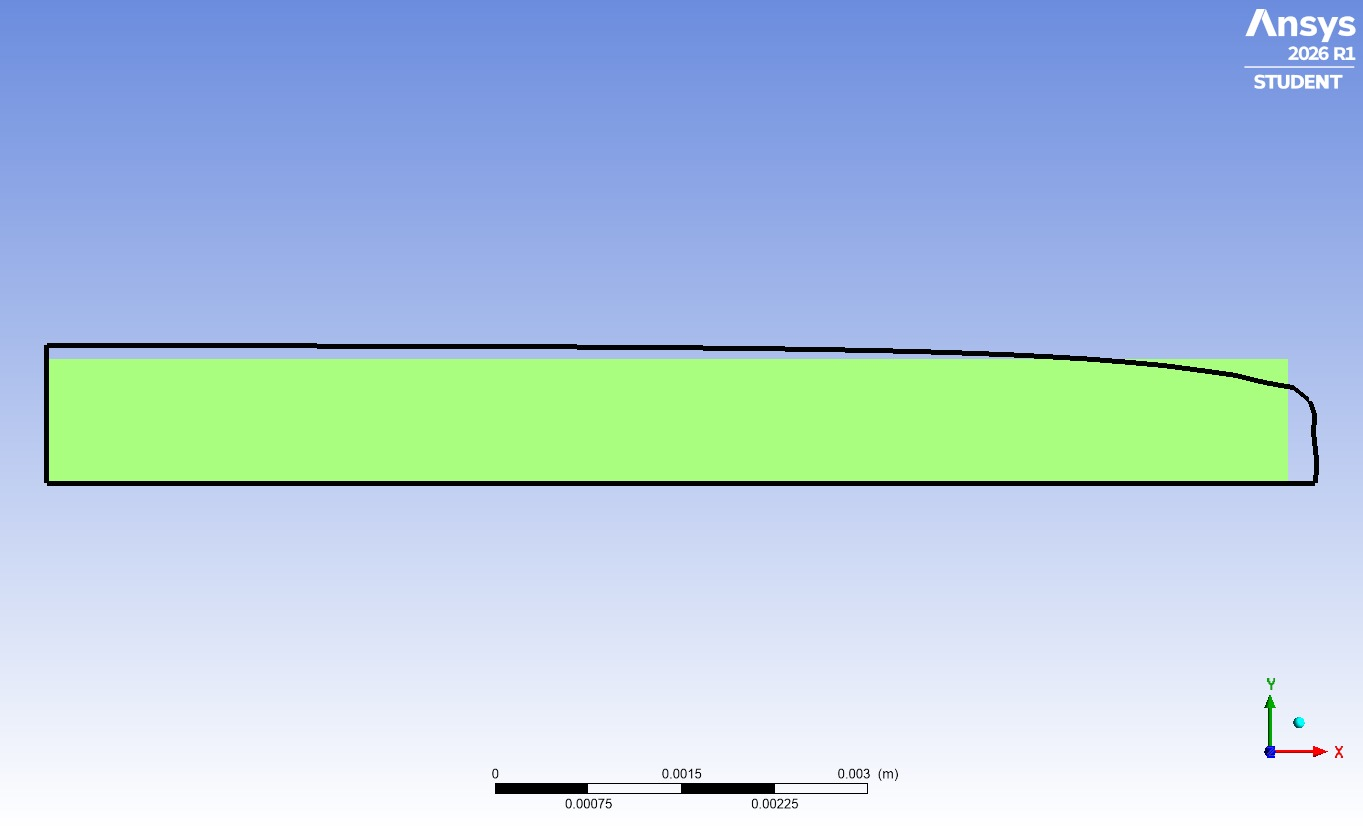
\includegraphics[width=\textwidth]{Imagens/perfil_M.jpeg}
        \caption{Caso M ($B_W = 1,023$; $B_H = 1,110$)}
        \label{fig:perfil_M}
    \end{subfigure}
    \caption{Contorno da secção transversal do extrudido em $z = 60\text{ mm}$ sobreposto à secção nominal da matriz: (a) Caso R e (b) Caso M.}
    \label{fig:inchamento}
\end{figure}

\subsection{Confronto com o Intervalo de Validade da Ficha Reológica}
\label{subsec:validade}

O modelo da lei de potência calibrado para o Moplen HP648T ($K = 900$~Pa$\cdot$s$^n$, $n = 0{,}64$) tem o seu intervalo de validade experimental circunscrito entre 60 e 500~s$^{-1}$, a 220~°C, conforme estipulado na ficha reológica~\cite{FichaMoplen}. A Figura~\ref{fig:validade_ficha} confronta esta janela de calibração com as taxas de deformação calculadas na simulação.

\begin{figure}[htbp]
    \centering
    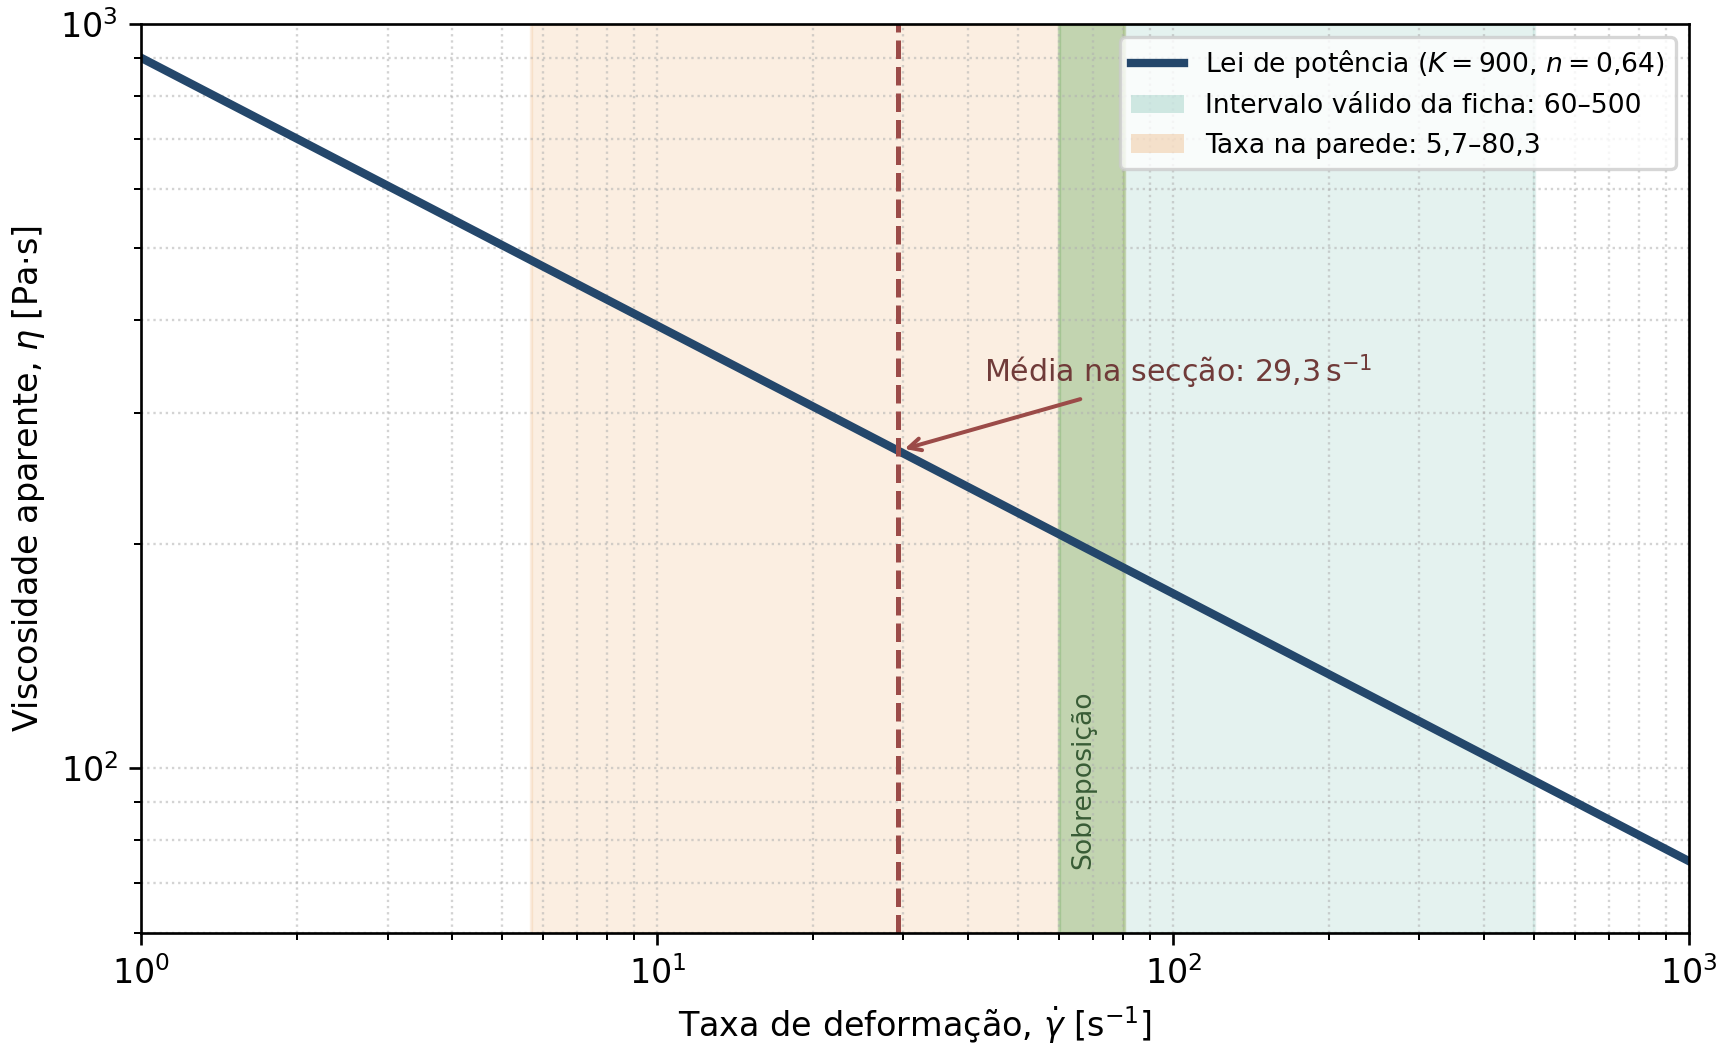
\includegraphics[width=0.72\textwidth]{Imagens/viscosidade_validade.png}
    \caption{Curva reológica do Moplen HP648T a 220~°C e confronto entre o intervalo de validade da ficha e a gama de taxas de deformação obtida no canal da matriz.}
    \label{fig:validade_ficha}
\end{figure}

A taxa de deformação na parede da matriz (DIEWALL) varia entre 5,7~s$^{-1}$, junto aos cantos, e 80,3~s$^{-1}$, no centro da parede larga. O valor médio na secção anterior à saída ($z = 19$~mm) é de apenas 29,3~s$^{-1}$. No núcleo central do canal e ao longo de todo o jato livre, o escoamento tende para velocidades uniformes e $\dot{\gamma}$ decai para valores próximos de zero.

Como se observa na Figura~\ref{fig:validade_ficha}, apenas uma fração estreita do escoamento junto às paredes largas opera dentro do intervalo válido da ficha, entre 60 e 80,3~s$^{-1}$. A maior parte do domínio opera por extrapolação da lei de potência para baixas taxas de corte ($\dot{\gamma} < 60$~s$^{-1}$). Como o modelo puramente potencial não contempla o patamar newtoniano ($\eta_0$), esta extrapolação sobrestima a viscosidade aparente nas regiões de menor cisalhamento, tendendo para $\eta \to \infty$ quando $\dot{\gamma} \to 0$. O limite superior de calibração (500~s$^{-1}$) não é ultrapassado em nenhum ponto do domínio.

\subsection{Quadro Síntese Comparativo (Caso R vs. Caso M)}
\label{subsec:sintese}

Na Tabela~\ref{tab:sintese_RM} apresentam-se e comparam-se as grandezas globais extraídas para o escoamento a caudal imposto ($Q = 2 \times 10^{-7}$~m$^3$/s no quarto do domínio), confrontando o fluido de referência (Caso R) com o polipropileno Moplen HP648T (Caso M). A variação relativa percentual é calculada por $(M-R)/R \times 100\%$.

\begin{table}[H]
    \centering
    \small
    \caption{Síntese dos resultados dos Casos R e M ($Q = 2 \times 10^{-7}$~m$^3$/s no quarto do domínio).}
    \label{tab:sintese_RM}
    \begin{tabular}{lccc}
        \toprule
        Grandeza & Caso R & Caso M & Variação ($M/R$) \\
        \midrule
        $\bar{p}_{\mathrm{ent}}$ [kPa] & 288,0 & 302,3 & $+5{,}0$\,\% \\
        $\bar{p}_{\text{saída}}$ [kPa] & 0,5 & 0,8 & $+53{,}5$\,\% \\
        $\Delta p$ [kPa] & 287,4 & 301,5 & $+4{,}9$\,\% \\
        $\dot{\gamma}_{\max}$ no domínio [s$^{-1}$] & 81,5 & 80,3 & $-1{,}5$\,\% \\
        $\dot{\gamma}$ médio em $z = 19$~mm [s$^{-1}$] & 29,1 & 29,3 & $+0{,}7$\,\% \\
        $\eta$ a $\dot{\gamma}_{\max}$ [Pa$\cdot$s] & 172 & 185 & $+7{,}6$\,\% \\
        $B_W$ [--] & 1,017 & 1,023 & $+0{,}6$\,\% \\
        $B_H$ [--] & 1,096 & 1,110 & $+1{,}3$\,\% \\
        $\varepsilon_Q$ [\%] & 0,009 & 0,009 & -- \\
        \bottomrule
    \end{tabular}
\end{table}

As pressões médias de entrada e saída e as respetivas variações estão arredondadas; os valores de $\Delta p$ e as percentagens foram calculados a partir dos resultados não arredondados.

A comparação da Tabela~\ref{tab:sintese_RM} mostra que a substituição do fluido de referência pelo Moplen HP648T aumenta a perda de carga em 4,9\,\%, acompanhada por um aumento de 7,6\,\% na viscosidade aparente à taxa de deformação máxima. Embora o fator de consistência do Caso M seja inferior ($K = 900$~Pa$\cdot$s$^n$, face a 1000~Pa$\cdot$s$^n$), o seu maior índice de comportamento reológico ($n = 0{,}64$, face a 0{,}60) corresponde a uma menor diminuição da viscosidade com o aumento da taxa de corte. Como $\eta = K\dot{\gamma}^{n-1}$, as viscosidades dos dois materiais cruzam-se perto de $\dot{\gamma} = 13{,}9$~s$^{-1}$: acima desse valor, a viscosidade do Caso M é superior; abaixo dele, a do Caso R é superior. Assim, não se verifica uma viscosidade maior do Caso M em toda a gama de taxas de corte.

Em termos cinemáticos, as taxas de deformação máxima e média permanecem praticamente inalteradas entre os casos (variações de $-1{,}5$\,\% e $+0{,}7$\,\%), indicando que a cinemática global é condicionada sobretudo pela geometria rígida da fieira e pelo caudal volumétrico imposto.

Quanto à resposta geométrica do extrudido, os rácios dimensionais $B_W$ e $B_H$ variam pouco em valor absoluto ($+0{,}6$\,\% e $+1{,}3$\,\%). Considerando o inchamento líquido acima das dimensões da matriz, calculado como $B-1$ a partir dos valores apresentados, a variação do Caso M face ao Caso R é de cerca de $+35$\,\% na largura ($0{,}023/0{,}017 \approx 1{,}35$) e $+15$\,\% na espessura ($0{,}110/0{,}096 \approx 1{,}15$), confirmando a maior propensão do material para a expansão pós-extrusão.

\section{Discussão e Decisão de Engenharia}




\subsection{Confronto Com as Previsões P1, P2, P3}



\subsection{Diferença Relevante Entre R e M e Efeito do Caudal}




\subsection{Limitações}



\subsection{Caracterização Adicional e Passo Seguinte}




\subsection{Decisão de Engenharia e Limite Científico}













%%%%%%%%%%%%%%%%%%%%%%%%%%%%%%%%%%%%%%%%%%%%%%%%%%%

\newpage

\phantomsection
\addcontentsline{toc}{part}{Elementos finais}
\newpage
\section*{Declaração de Utilização de Inteligência Artificial}
\phantomsection
\addcontentsline{toc}{section}{Declaração de Utilização de Inteligência Artificial}
\noindent\textbf{Ferramenta(s):} Claude; Gemini; Consensus \\[1.5em]
\textbf{Finalidade:} Apoio na redação e na revisão de texto e deteção de inconsistências no relatório. \\[1.5em]
\noindent\textbf{Contributo utilizado:}
\begin{itemize}
    \item Rascunhos de texto, que o grupo reescreveu antes de os incluir.
    \item Identificação de inconsistências entre secções do relatório.
    \item Checklist de conclusão do relatório face ao enunciado do portefólio.
    \item Revisão ortográfica e gramatical de texto do relatório.
    \item Pesquisa científica de artigos
\end{itemize}



\noindent\textbf{Como foi verificado pelo grupo:} Todos os valores numéricos, parâmetros térmicos extraídos no software TRIOS ($T_{\mathrm{m}}$, $T_{\mathrm{c}}$, $\Delta H$) e cálculos derivados ($X_{\mathrm{c}}$, médias e desvios-padrão de MFR) foram conferidos manualmente pelo grupo contra os ficheiros originais de ensaio e as folhas de cálculo. As sugestões de texto e estrutura geradas pelas ferramentas foram criticamente revistas, adaptadas e reformuladas pelos autores, garantindo que as interpretações físicas, as fontes bibliográficas consultadas e as decisões de engenharia refletem exclusivamente a análise e a responsabilidade técnica do grupo.

\newpage

\phantomsection
\addcontentsline{toc}{section}{\refname}
\bibliographystyle{unsrtnat}
\bibliography{metodologia}



\newpage
\appendix





\end{document}
